% !TeX program = pdflatex
%==============================================================================
%  Aula E3 --- NLP + Classificação (Aplicação)
%  VERSÃO DO ALUNO: texto para leitura autônoma, fora da sala.
%  (O roteiro de sala é "E3 NLP e Classificacao.tex".)
%==============================================================================
\documentclass[11pt,a4paper]{article}
\usepackage[aluno]{../../recursos/latex/estilo-notas}

\title{}
\date{}

\begin{document}
\cabecalhoaula{Extra E3}{NLP $+$ Classificação (Aplicação)}{Aplicação (notebook); AME §8.1.3 e Ap.~A.2--A.3}

%==============================================================================
\section*{O que você vai aprender}
%==============================================================================
Ao final desta aula você deve ser capaz de:
\begin{itemize}[leftmargin=1.4cm]
  \item descrever as etapas de limpeza e normalização de texto;
  \item construir a \textbf{matriz documento--termo} (\emph{bag-of-words}) e explicar
        por que ela é esparsa;
  \item definir o \textbf{TF--IDF} e dizer o que ele corrige;
  \item escolher métodos adequados a alta dimensão esparsa e justificar a escolha
        pela teoria da Aula~05;
  \item avaliar um classificador de \emph{spam} com as métricas certas (Aula~09);
  \item montar o \emph{pipeline} completo, sem vazamento (Aula~07).
\end{itemize}

\noindent
Esta é a última aula do curso, e ela não traz nenhum método novo: traz um
\emph{problema} novo, e mostra que as ferramentas dos onze encontros anteriores já
dão conta dele. A pergunta:

\begin{center}\itshape
  um modelo só entende números. Como transformar uma mensagem de texto\\
  em covariáveis?
\end{center}

%==============================================================================
\section{O problema: filtrar spam}
%==============================================================================
Usaremos a base \texttt{spam.csv} (SMS Spam Collection): $5\,572$ mensagens de
SMS rotuladas como \emph{ham} (legítima, $Y=0$) ou \emph{spam} ($Y=1$), sendo
$13{,}4\%$ delas \emph{spam}. É um problema de \textbf{classificação binária}
(Aula~08) cujas covariáveis são \emph{texto bruto} --- e o desafio central é a
\emph{representação}.

\begin{atencao}
A base é \textbf{desbalanceada}. Como vimos na Aula~09, a acurácia engana aqui: um
classificador que declarasse tudo \emph{ham} já acertaria $86{,}6\%$. Precisaremos de
precisão, \emph{recall} e $F_1$. E os custos são assimétricos: bloquear uma mensagem
legítima (falso positivo) costuma ser bem pior que deixar passar um \emph{spam} ---
o que, pela Proposição~4.1 da Aula~09, significa exigir um corte \emph{alto} para
declarar \emph{spam}.
\end{atencao}

%==============================================================================
\section{Do texto aos atributos}
%==============================================================================
\subsection{Limpeza e normalização}
Texto bruto é ruidoso. As etapas usuais de pré-processamento:
\begin{itemize}[leftmargin=1.4cm,nosep]
  \item \emph{minusculizar} (\texttt{lower}): ``Free'' e ``free'' viram o mesmo
        \emph{token};
  \item remover \textbf{pontuação} e \textbf{números} (conforme o problema);
  \item \emph{tokenizar}: quebrar a mensagem em palavras (\emph{tokens});
  \item remover \textbf{\emph{stopwords}}: palavras muito frequentes e pouco
        informativas (``the'', ``is'', ``and'');
  \item \emph{stemming}/\emph{lematização} (opcional): reduzir flexões a um radical
        (``running'' $\to$ ``run'').
\end{itemize}

\begin{atencao}
Cada uma dessas etapas \emph{descarta informação}, e nem sempre a informação certa.
Remover números destrói ``ganhe R\$ 1000'', que é justamente um sinal de
\emph{spam}; minusculizar apaga ``GRÁTIS'' gritado em maiúsculas. Não aplique a
lista por reflexo: cada decisão é um hiperparâmetro, e vale testá-la por validação
cruzada como qualquer outro.
\end{atencao}

\subsection{\emph{Bag-of-words} e a matriz documento--termo}
A representação mais simples é o \textbf{\emph{bag-of-words}} (saco de palavras):
ignora-se a ordem e conta-se a ocorrência de cada palavra. Constrói-se a
\textbf{matriz documento--termo} $\bm{X}$, em que a linha $i$ é a mensagem $i$, a
coluna $j$ é um termo do vocabulário, e $x_{ij}$ é a contagem (ou presença binária)
do termo $j$ na mensagem $i$.

\begin{figure}[htbp]
  \centering
  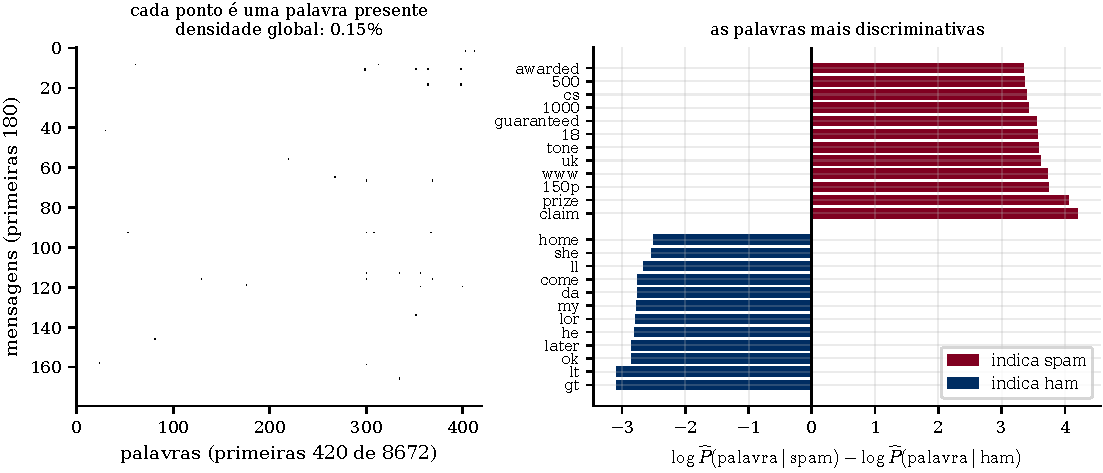
\includegraphics[width=\textwidth]{../../recursos/figuras/E3-texto.pdf}
  \caption{À esquerda, um pedaço da matriz documento--termo da base
  \texttt{spam.csv}: cada ponto preto é uma palavra presente numa mensagem. A matriz
  completa tem $5\,572$ linhas e $8\,672$ colunas, e apenas $0{,}15\%$ das
  posições são não nulas --- em média $13$ palavras distintas por mensagem, de um
  vocabulário de quase nove mil. À direita, as palavras que mais deslocam a decisão
  de um Bayes ingênuo multinomial: de um lado ``claim'', ``prize'', ``150p'',
  ``www''; do outro, o vocabulário do dia a dia.}
  \label{fig:texto}
\end{figure}

\begin{ideia}
Repare na desproporção que a figura registra: $5\,572 \times 8\,672$ dá quase $48$
milhões de posições, das quais só umas $74$ mil são não nulas. Guardar essa matriz
densamente desperdiça mais de $99\%$ da memória --- daí os \textbf{formatos
esparsos} (Apêndice~A.3 do [AME]), que armazenam apenas as posições ocupadas. O
\texttt{scikit-learn} devolve matrizes esparsas por padrão nos vetorizadores, e é
por isso que o problema é tratável num laptop.
\end{ideia}

\begin{atencao}[Eis a Aula~05 em ação]
Texto é o exemplo canônico de \textbf{alta dimensão $+$ esparsidade}: milhares de
palavras, mas a maioria irrelevante para a classe. Por isso métodos que
\emph{selecionam variáveis} (Lasso, Bayes ingênuo) vão bem, e o KNN vai mal --- ele
não seleciona, e a distância euclidiana entre duas mensagens é dominada pelas
milhares de palavras que nenhuma das duas contém. É \emph{literalmente} a pergunta
da Amazon que abriu a Aula~05, agora com os dados na mão.
\end{atencao}

\subsection{TF--IDF}
Contagens cruas dão peso demais a palavras comuns. O \textbf{TF--IDF}
(\emph{term frequency--inverse document frequency}) reescala cada termo:
\[
  \text{tf-idf}(t,d) = \underbrace{\text{tf}(t,d)}_{\substack{\text{frequência do termo}\\\text{no documento }d}}
  \times
  \underbrace{\log\frac{N}{\text{df}(t)}}_{\substack{\text{raridade do termo}\\\text{na coleção}}},
\]
onde $\text{df}(t)$ é o número de documentos que contêm $t$ e $N$ o total. Palavras
que aparecem em \emph{todo} documento têm IDF baixo (pouco discriminantes); palavras
\emph{raras e específicas} ganham peso.

\begin{ideia}
O IDF é uma versão automática da remoção de \emph{stopwords}, e melhor: em vez de
usar uma lista fixa, ele descobre \emph{nos seus dados} quais palavras são comuns
demais para informar. Se aparece em todo documento, $\text{df}(t)=N$, o logaritmo
zera e a palavra some sozinha. É o mesmo espírito do Lasso na Aula~02 --- deixar os
dados decidirem o que descartar.
\end{ideia}

%==============================================================================
\section{Análise exploratória}
%==============================================================================
Antes de modelar, vale \emph{olhar} os dados: quais as palavras mais frequentes em
\emph{ham} \emph{versus} \emph{spam}? O painel direito da Figura~\ref{fig:texto}
responde de forma quantitativa, ordenando as palavras por
$\log\widehat\Prob(\text{palavra}\mid\text{spam})-
 \log\widehat\Prob(\text{palavra}\mid\text{ham})$. Do lado do \emph{spam} aparecem
``claim'', ``prize'', ``guaranteed'', ``150p'', ``www'', ``uk'', ``1000'' --- o
vocabulário de promoções e números de tarifação. Do lado do \emph{ham}, palavras
banais de conversa. Esse contraste já mostra que o \emph{bag-of-words} carrega
sinal suficiente para separar as classes, antes de ajustar qualquer modelo.

%==============================================================================
\section{Classificando}
%==============================================================================
Quais métodos usar? Os que prosperam em alta dimensão esparsa:
\begin{description}[leftmargin=2.8cm,style=nextline]
  \item[Bayes ingênuo (multinomial)] o ``cavalo de batalha'' do texto. A suposição
        de independência condicional (Aula~08) é grosseira para palavras --- ``prize''
        e ``win'' claramente andam juntas --- mas funciona surpreendentemente bem e é
        rápida. A versão \emph{multinomial} modela contagens. (Lembre da Aula~08:
        trabalhe em escala logarítmica para evitar \emph{underflow}.)
  \item[Logística penalizada (Lasso/Ridge)] discriminativa, robusta, e o Lasso faz
        \emph{seleção de palavras} --- gerando um modelo interpretável (quais
        palavras pesam para \emph{spam}). É o que o [AME] usa no exemplo das resenhas
        da Amazon.
  \item[Florestas / \emph{boosting}] também aplicáveis; XGBoost costuma ir bem.
\end{description}

\begin{ideia}
Por que Bayes ingênuo combina tão bem com texto? Porque o modelo multinomial sobre
contagens é natural, há pouquíssimos parâmetros por palavra (baixa variância) e a
independência condicional, embora falsa, raramente troca a \emph{classe} de maior
probabilidade --- e, para classificar, basta acertar o lado do corte.
\end{ideia}

\begin{atencao}
Mas atenção ao que a Aula~09 mediu: o Bayes ingênuo com covariáveis correlacionadas
--- e palavras \emph{são} correlacionadas --- produz probabilidades muito
descalibradas, mesmo classificando bem. Se você for ajustar o corte por custos
(como o problema de \emph{spam} pede), estará mexendo justamente nos números em que
não se pode confiar. Nesse caso, ou use a logística, ou calibre o Bayes ingênuo com
\texttt{CalibratedClassifierCV}.
\end{atencao}

%==============================================================================
\section{Avaliação}
%==============================================================================
Como o problema é desbalanceado (Aula~09):
\begin{itemize}[leftmargin=1.4cm,nosep]
  \item reporte a \textbf{matriz de confusão}, \textbf{precisão}, \textbf{\emph{recall}}
        e \textbf{$F_1$} --- não só a acurácia;
  \item para \emph{spam}, a \emph{precisão} sobre a classe ``spam'' é crítica:
        precisão alta significa que quase tudo que você bloqueou era mesmo lixo;
  \item ajuste o \textbf{corte} de decisão conforme os custos: se um falso positivo
        é dez vezes mais caro que um falso negativo, o corte ótimo é
        $10/11\approx0{,}91$, não $0{,}5$.
\end{itemize}

%==============================================================================
\section{O \emph{pipeline} completo (síntese do curso)}
%==============================================================================
Tudo se encaixa num único \emph{pipeline} (Aula~07): vetorização $\to$ classificador,
com hiperparâmetros escolhidos por validação cruzada (Aula~03) \emph{sem vazamento}
--- e o vetorizador deve aprender o vocabulário \textbf{só no treino}.

\begin{lstlisting}
import pandas as pd
from sklearn.feature_extraction.text import CountVectorizer, TfidfVectorizer
from sklearn.naive_bayes import MultinomialNB
from sklearn.linear_model import LogisticRegression
from sklearn.pipeline import Pipeline
from sklearn.model_selection import train_test_split, GridSearchCV
from sklearn.metrics import classification_report, confusion_matrix

sms = pd.read_csv("spam.csv", encoding="ISO-8859-1")
X, y = sms["text"], (sms["class"] == "spam").astype(int)
X_tr, X_te, y_tr, y_te = train_test_split(X, y, test_size=0.3,
                                          stratify=y, random_state=0)

# vetorizacao + classificador num unico objeto (sem vazamento!)
pipe = Pipeline([
    ("vec", TfidfVectorizer(lowercase=True, stop_words="english")),
    ("clf", MultinomialNB()),
])
grade = {"vec__ngram_range": [(1,1), (1,2)],
         "clf__alpha":       [0.1, 0.5, 1.0]}     # suavizacao de Laplace
busca = GridSearchCV(pipe, grade, cv=5, scoring="f1").fit(X_tr, y_tr)

y_hat = busca.predict(X_te)
print(confusion_matrix(y_te, y_hat))
print(classification_report(y_te, y_hat))        # precisao, recall, F1
\end{lstlisting}

\begin{atencao}[por que o vetorizador \emph{tem} que estar no pipeline]
Se você vetorizar tudo antes de separar treino e teste, o vocabulário --- e os
valores de IDF --- serão calculados usando as mensagens de teste. É vazamento da
categoria \textbf{grave} da Aula~07: uma etapa que \emph{escolhe} quais colunas
existem, olhando dados que deveriam ser novos. Dentro do \emph{pipeline}, cada
dobra reconstrói o vocabulário do zero, e palavras que só aparecem no teste são
simplesmente ignoradas --- que é exatamente o que aconteceria em produção.
\end{atencao}

\begin{observacao}[o que \emph{não} vimos]
O \emph{bag-of-words} joga fora a ordem das palavras: para ele, ``não é spam'' e
``é spam não'' são idênticos. Métodos modernos de NLP --- \emph{embeddings},
redes recorrentes, \emph{transformers} --- existem justamente para recuperar essa
informação, e estão fora do escopo do curso ([ISLP] §10.4--10.5 dá uma introdução).
Vale saber que, para muitas tarefas de classificação de texto, a diferença de
desempenho entre um TF--IDF com logística e um modelo grande é menor do que se
imagina --- e o primeiro roda em segundos e você consegue explicar.
\end{observacao}

O notebook \texttt{Aula prática E3} percorre a limpeza, a exploração
e a classificação na base \texttt{spam.csv}.

%==============================================================================
\section*{Resumo (e encerramento do curso)}
%==============================================================================
\begin{itemize}[leftmargin=1.4cm]
  \item Texto vira número pelo \emph{bag-of-words}: matriz documento--termo,
        gigantesca e \textbf{esparsa} --- $0{,}15\%$ de posições ocupadas na nossa
        base (Fig.~\ref{fig:texto}).
  \item Limpeza e normalização descartam informação: trate as escolhas como
        hiperparâmetros.
  \item \textbf{TF--IDF} reescala pela raridade, descontando automaticamente as
        palavras comuns demais.
  \item Alta dimensão $+$ esparsidade $\Rightarrow$ Bayes ingênuo e logística
        penalizada; KNN vai mal, pelo motivo da Aula~05.
  \item Avalie com precisão/\emph{recall}/$F_1$ e ajuste o corte pelos custos
        (Aula~09); cuidado com a calibração do Bayes ingênuo.
  \item Tudo num \emph{pipeline} (Aula~07): o vetorizador aprende o vocabulário
        \emph{só} no treino.
\end{itemize}

\noindent
E é assim que o curso fecha. Este problema não exigiu nenhuma ideia que você já não
tivesse: a representação veio da Aula~07, a escolha do método veio da teoria da
Aula~05, o classificador veio da Aula~08, a avaliação veio da Aula~09 e a montagem
sem vazamento veio da Aula~03. O arcabouço da Aula~01 --- risco, viés--variância,
seleção de modelos --- continua sendo o mesmo, quer as covariáveis sejam a
temperatura crítica de um supercondutor ou as palavras de um SMS.

\paragraph{Leitura recomendada.} [AME] §8.1.3 (Bayes ingênuo), §3.8 e §8.8 (os
exemplos com as resenhas da Amazon, que são a versão em regressão e em classificação
do que fizemos aqui), Apêndice~A.2 (manipulação de textos) e A.3 (matrizes
esparsas). [ISLP] §10.4 (\emph{Document Classification}), para ver o mesmo problema
tratado com redes neurais. Documentação do \texttt{scikit-learn}: \emph{Working With
Text Data}, que é um tutorial completo e curto.

\paragraph{Para praticar.} \texttt{Lista teorica E3.pdf} (teórica, com gabarito) e \texttt{Lista prática E3.ipynb} (prática, para completar as lacunas), nesta mesma pasta.

\end{document}
